\chapter{Game programming concepts overview}
\label{chapter:Chapter 3}

In this chapter I’m going to introduce a few game programming concepts.

\section{Primitives}

\subsection{Triangles}

The smallest three dimensional primitive available, any polygon can be split into triangles. GPUs work by rendering triangles, they are the basic unit which they process. Another advantage of a triangle is that it is always planar; this is only true for triangles, any polygon with more than three vertices can have its fourth vertex not in the same plane as defined by the first three. No matter what transformation you apply to a triangle it will remain a triangle, at most you can get an edge case in which it is a single line.
The last advantage, as mentioned in the GameEngineArhitecture (from reference \cite{gregory09}), it is the basic shape that all 3D accelerators render and it has been used in the gaming industry even from the first 3D games like Castle Wolfenstein and Doom.

Triangles can be given to the GPU in many ways. Each triangle must be defined by three points in space, its vertices.

\subsubsection{Winding Order}

Each of the triangles have a winding order specified by the order in which the vertices of the triangle are specified. Each vertice is specified using a vector. From these we calculate the vectors for each edge:
\[ \mathbf{e}_{12} = p_{2} - p_{1}\]
\[ \mathbf{e}_{13} = p_{3} - p_{1}\]
\[\mathbf{e}_{23} = p_{3} - p_{2}\]

The face normal, N, is defined using the normalized cross product of any two edges:

\[ N = \frac{\mathbf{e}_{12}\times \mathbf{e}_{13}}{\left | \mathbf{e}_{12}\times \mathbf{e}_{13}  \right |}\]

The normal is necessary in order to figure out which is the front face and which is the back, the reason we need this is so that OpenGL can do back face culling. This is especially required for transparent objects.

\subsubsection{Triangle lists, indexed traingle lists, strips and fans}

There are multiple ways of specifying triangles to the GPU. Here are four ways in which we can do this using OpenGL:

\textbullet Triangle Lists - The most simple way of specifying triangles for the videocard to render is by using a triangle list. This is a list of points, each three points making a triangle with the winding order in the order in which they are specified.

\textbullet Indexed Triangle Lists -  If a object shares points with multiple triangles it is easier to specify a list o points and another list of indexes for the order in which the points form triangles.

\textbullet Triangle Strips - These can be used for rendering a triangle strip in which a point always forms a triangle with the previous two points. These specialized structures can be used to efficiently store a mesh, since it doesn’t require repeating vertices and also it doesn’t need a index buffer.

\textbullet Triangle Fans - Triangle fans are similar to strips, just that they make a triangle with the first vertice in the fan and the last one.

\subsection{Model space}

Model space is the space defined in respect to a local location, like the parent object. It is used in order to reference the position of the triangles in a mesh. Each object has it’s own model space.

\subsection{World space}

World space is the space for an entire scene. A scene is usually made up of multiple models. In order to convert vertices from model space to world space, a transformation matrix is used, often called world matrix. This matrix contains rotation, scaling and transformation into a single matrix.

\subsection{View space}

View space is the space which the camera sees. The view space is centered in the camera’s focal point. It is usually obtained by multiplying the world space with the camera’s projection matrix and the camera’s view matrix. The camera projection matrix calculates.

\section{Mathemathics}

There are a couple of mathematical concepts that are required in order to understand the concepts.

\subsection{Matrices}

Matrices are used in order to efficiently apply transformations to vertices. There are 3 types of transformation that can be done using matrices.

\subsubsection{Translation}

Translation matrices are used in order to translate an object to another position. These matrices look like:

\[ \begin{bmatrix}
	1 & 0 & 0 & v_{x}\\ 
	0 & 1 & 0 & v_{y}\\ 
	0 & 0 & 1 & v_{z}\\ 
	0 & 0 & 0 & 1
\end{bmatrix}
\]

The \(v_{x}\), \(v_{y}\) and \(v_{z}\) represent the amount of movement under the respective axes.

\subsubsection{Rotation}

For rotation there are three rotation matrices, each for each axis:

% insert matrices here

\subsubsection{Scaling}

Scaling matrices are used for scaling coordinates to the same scale.

 % insert matrices here
 
This allows each axis to be scaled individually. If all axis are scaled with the same factor, a simplified matrix can be used:
 
 % insert matrices here
 
Where s is the scaling factor, because the last coordinate can be viewed as the denominator for the other three coordinates.
 
\subsection{Quaternions}

\section{Rendering pipeline}

WebGL’s rendering pipeline is the same as OpenGL ES 2.0’s since the specification was made after it. As can be seen from the figure ~\ref{img:opengles1}, the pipeline figures just two programmable points the Vertex Shader and the Fragment Shader. All the others are fixed hardware operations. \footnote{http://www.khronos.org/api/opengles/2\_X}

 \begin{center}
	\begin{figure}[here]
		
		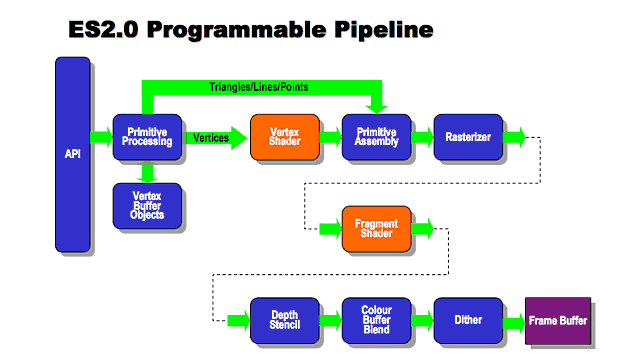
\includegraphics[width=\textwidth]{src/img/opengles2.png}
		\caption{Programmable Pipeline}
		\label{img:opengles1}
	\end{figure}
\end{center}

\section{Rendering techniques}

\subsection{Forward rendering}

Forward rendering is the default type of rendering. In forward rendering meshes are rendered on the GPU in the order in which they are sent. Special care must be taken when rendering transparent materials, as these must be rendered at the end. The forward renderer 

\subsection{Deferred Rendering}

With the advances in OpenGL ES 2.0 and the porting of these improvements to WebGL specific extensions, advanced rendering technique (that were previously only used in desktop based implementations) became available.(from reference \cite{engel14}) This chapter presents advances in deferred rendering using OpenGL ES 2 and how to adapt them for working on WebGL. 

There are 3 main deferred rendering techniques used in the industry. The first one is deferred rendering, as presented by Nvidia and implemented in S.T.A.L.K.E.R. Engine. The second technique is Light Indexed Rendering, used in engines like DOOM 3 engine; \cite{trebilco07} it is an approach which permits the use of forward rendering while doing a precalculation of lighting information.

The last and most modern approach is known as light pre-pass rendering or deferred lighting. It was first introduced by Wolfgang Engel (\cite{engel08}) and it is an approach more appropriate for modern GPUs, which don’t lack the compute power but lack the memory bandwidth, solving the problem of materials in deferred rendering.

\subsubsection{Deferred rendering}

Deferred rendering is based on rendering the scene and saving in a frame buffer all the information necessary for calculating lighting. The name “deferred” comes from the fact that no shading is calculated in the first pass, it is “deferred” to the second pass. Position, normals, ambient light and materials for each surface are rendered into the geometry buffer (G-buffer) as a series of textures. After these textures are rendered, a new pass renders the lights as various shapes (cones for spotlight and spheres for point lights) and together with the information contained in the G-Buffer, renders the scene. The only major problem is that material information must also be stored in the G-Buffer, this making the G-Buffer increase in size a lot. This was not practical for last gen consoles, so a different rendering method was necessary, as seen in ~\ref{img:deferred2}.
\begin{center}
\begin{figure}[here]
	
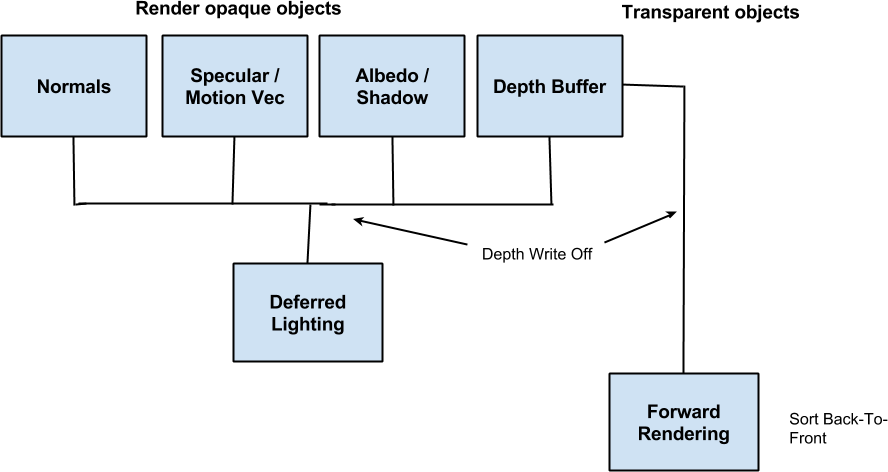
\includegraphics[width=\textwidth]{src/img/deferred2.png}
\caption{Deferred rendering using a G-Buffer}
\label{img:deferred2}
\end{figure}
\end{center}

An example of a G-Buffer taken from the presentation of the Killzone 2 engine can be seen in figure ~\ref{img:deferred1}.

\begin{center}
	\begin{figure}[here]
		
		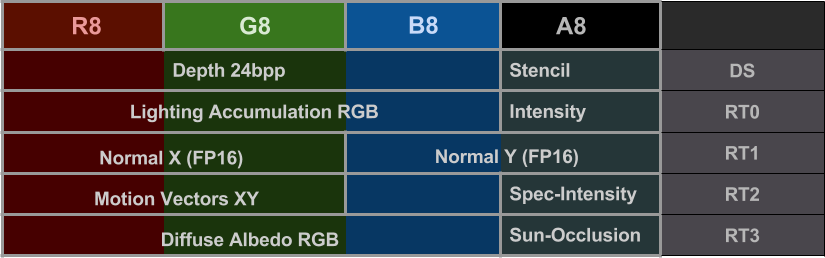
\includegraphics[width=\textwidth]{src/img/deferred1.png}
		\caption{G-Buffer from Killzone 2 engine}
		\label{img:deferred1}
	\end{figure}
\end{center}

\subsubsection{Deferred lighting}

Deferred lighting or light pre-pass deferred rendering works by rendering in a first phase a minimal G-Buffer which contains only normals and depth information. After this pass, a second pass is done in which lights are rendered similar to the deferred rendering second phase, just that instead of rendering the final scene, the light information is stored in a frame buffer. 
Another pass is necessary in order to obtain the final scene. In this pass, the geometry is rendered again and the information from the light pass is used in order to calculate the lighting.
The main advantage over deferred rendering is that it supports different material and a smaller G-Buffer, but it requires that the geometry be rendered again. The bandwidth cost is not that different, 5 buffer passes compared to 6 for deferred rendering.
It still needs another forward pass in order to render transparent objects.~\ref{img:lightning1}

\begin{center}
	\begin{figure}[here]
		
		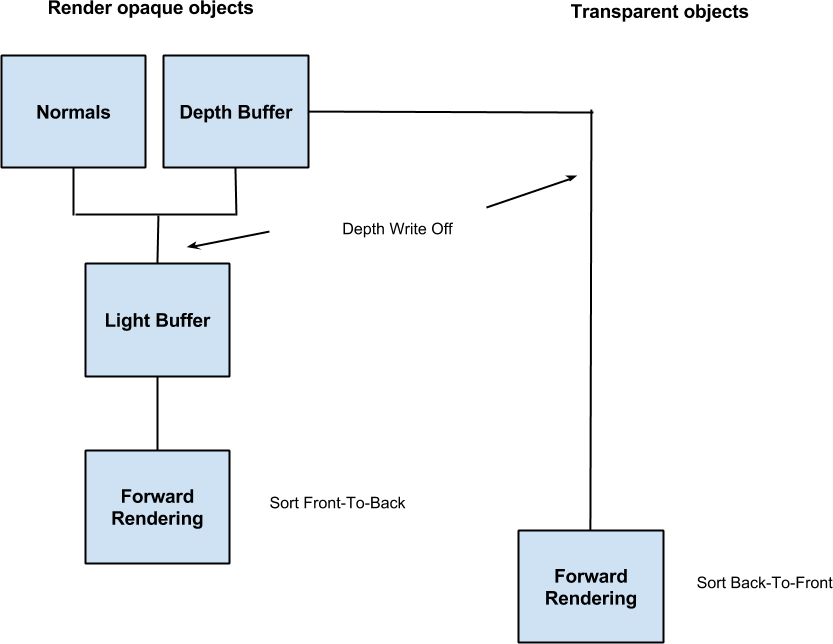
\includegraphics[scale=0.3]{src/img/lightning1.png}
		\caption{Renderer layout}
		\label{img:lightning1}
	\end{figure}
\end{center}

\subsubsection{Light indexed rendering}

In light indexed rendering, the first thing rendered are the light volumes. Each light has a certain id which, if encoded on a byte, can be up to 255 (meaning we can have 256 individual lights on a scene). The index is written to the texture in a specific channel using glColorMask, which allows for up to four lights for a standard RGBA8 texture.
In the next pass, the scene geometry is rendered and using information from the light index texture, lighting is computed.
Due to the large number of lights, lighting information must be kept in separate textures.
The only limitation of this technique is that no more than four lights can cover the same pixel, but if it requires more than four then you can use more textures. If more than 256 lights are required, the textures can be changed to bigger ones like RGBA16, giving you 65536 lights. But this increases the bandwidth used and the memory used for storage.
The major advantage of this rendering method is that this is only forward rendering, meaning that there is no separate pass required for rendering transparent objects.

\section{Resource management}

\subsection{Assimp}

Open Asset Import Library (assimp) is an open source library that imports 41 types of assets and offers a common API for accessing them. It is licensed under BSD license, thus making it easily usable in commercial products. The library also does post processing by computing normals and tangent vectors when they are not available in the format, or by loading native textures from the format. There isn’t a port of this library to JavaScript but there is another project named assimp2json that outputs a json format of the files. This json has the same format as the API offered by assimp to other programming languages like C/C++, C\#/.net, Python and D.  Assimp can be used either offline in the asset conditioning pipeline or at runtime in the resource manager.

\subsection{Runtime Resource Management}

Different engines use different resource managers at runtime. These resource managers work tightly with the asset pipeline used to produce the resource files.
The most simple resource manager will load resources from a folder on disk. Each resource will be identified by their relative path. One problem is that usually operating systems inquire a cost of accessing a file on disk. Other engines will pack together assets and use a virtual filesystem for accessing the files. For example, in Game Engine Architecture the author gives as an example the Ogre3D engine which uses a large zip archive to store the contents of the game.





